% $Id: template.tex 11 2007-04-03 22:25:53Z jpeltier $

\documentclass{vgtc}                          % final

%%
\ifpdf%                                % if we use pdflatex
  \pdfoutput=1\relax                   % create PDFs from pdfLaTeX
  \pdfcompresslevel=9                  % PDF Compression
  \pdfoptionpdfminorversion=7          % create PDF 1.7
  \ExecuteOptions{pdftex}
  \usepackage{graphicx}                % allow us to embed graphics files
  \DeclareGraphicsExtensions{.pdf,.png,.jpg,.jpeg} % for pdflatex we expect .pdf, .png, or .jpg files
\else%                                 % else we use pure latex
  \ExecuteOptions{dvips}
  \usepackage{graphicx}                % allow us to embed graphics files
  \DeclareGraphicsExtensions{.eps}     % for pure latex we expect eps files
\fi%

%% it is recomended to use ``\autoref{sec:bla}'' instead of ``Fig.~\ref{sec:bla}''
\graphicspath{ {.} } % where to search for the images

\usepackage{microtype}                 % use micro-typography (slightly more compact, better to read)
\PassOptionsToPackage{warn}{textcomp}  % to address font issues with \textrightarrow
\usepackage{textcomp}                  % use better special symbols
\usepackage{mathptmx}                  % use matching math font
\usepackage{times}                     % we use Times as the main font
\renewcommand*\ttdefault{txtt}         % a nicer typewriter font
\usepackage{cite}                      % needed to automatically sort the references
\usepackage{tabu}                      % only used for the table example
\usepackage{booktabs}                  % only used for the table example
\usepackage{hyperref}
\usepackage{color}
%% If you are submitting a paper to a conference for review with a double
%% blind reviewing process, please replace the value ``0'' below with your
%% OnlineID. Otherwise, you may safely leave it at ``0''.
\onlineid{0}

%% declare the category of your paper, only shown in review mode
\vgtccategory{Research}

%% allow for this line if you want the electronic option to work properly
\vgtcinsertpkg

%% In preprint mode you may define your own headline.
%\preprinttext{To appear in an IEEE VGTC sponsored conference.}

%% Paper title.

\title{Interactive Visualization of Global Economy Growth}

%% Author and Affiliation (multiple authors with multiple affiliations)
\author{Zong Fan\thanks{e-mail: zongfan2@illinois.com}\\ %
        \scriptsize UIUC Bioengineering} %

%% A teaser figure can be included as follows, but is not recommended since
%% the space is now taken up by a full width abstract.
%\teaser{
%  \includegraphics[width=1.5in]{sample.eps}
%  \caption{Lookit! Lookit!}
%}

%% Abstract section.
\abstract{
Since 1990s, the end of the cold war, economic development has been the major concern of most countries around the world. The economic development status could usually reflect the success of political and economic policy. To learn from those highly-developed and fast-growing countries is an important method to promote the progress of human society and eliminate poverty. Therefore, in order to better understand the economy status of each country, we have developed an interactive interface to visualize economic data on the world map.%
} % end of abstract

\CCScatlist{
  \CCScatTwelve{User Interfaces}{User Interfaces}{Graphical user interfaces (GUI)}{}
}

%% Copyright space is enabled by default as required by guidelines.
%% It is disabled by the 'review' option or via the following command:
% \nocopyrightspace

%%%%%%%%%%%%%%%%%%%%%%%%%%%%%%%%%%%%%%%%%%%%%%%%%%%%%%%%%%%%%%%%
%%%%%%%%%%%%%%%%%%%%%% START OF THE PAPER %%%%%%%%%%%%%%%%%%%%%%
%%%%%%%%%%%%%%%%%%%%%%%%%%%%%%%%%%%%%%%%%%%%%%%%%%%%%%%%%%%%%%%%%

\begin{document}

%% The ``\maketitle'' command must be the first command after the
%% ``\begin{document}'' command. It prepares and prints the title block.

%% the only exception to this rule is the \firstsection command
\firstsection{Introduction}

\maketitle

%% \section{Introduction} %for journal use above \firstsection{..} instead
To evaluate a country's economic activity, one most important indicator is Gross Domestic Product (GDP) \cite{Jacob:2019:gdp}. GDP measures the value created through the production of goods and services in a country during a certain period of time. However, there are multiple rules to measure GDPs which vary among different countries. In order to get a relatively reliable GDP data to make comparison, we would refer to  national accounts data provided by the World Bank, who calls for value added to be valued at either basic prices excluding net taxes on products or producer prices including net taxes on products \cite{worldbank:2020:gdp}. Since 1960, the World Bank has already released GDP data of each country annually in current U.S. dollars. With this collected GDP data over the last 60 years, it's very convenient and useful for economists or policy-makers to review the comprehensive status quo of development around the world and the trend of particular country or region for determining future policies. 

With this set of GDP data, we are more interested in the GDP growth pattern after 1990. The end of the Cold War is a milestone in globalization which causes profound changes on current global economic landscape. It's interesting to find answers towards to following questions: which countries had the largest GDP? How the world's GDP changed overtime? what's the detailed trend of GDP development of a particular country? Since we need to analyze data from over 200 countries and 30 years, it's difficult to capture important information immediately from the raw data. Therefore, we developed an interactive webpage interface based on a Python package called Bokeh \cite{bokeh:2018} to help us visually discern the interesting patterns on world map more easily. 

\section{Visualize GDP on World Map}
Since we need to apply visual analytics on all countries on the world, it's straightforward to map the country's GDP data on its corresponding geometric location on the world map. We first use the geometric data provided by Natural Earth\cite{natrualearth:2018} to draw the world map. The geometric data together with associated attribute information are stored in shapefile format comprising a set of vector coordinates\cite{esri:1998:shapefile}. Then we retrieve GDP data of each country downloaded from World Bank database and use linear colormap to assign a particular color from viridis colormap based on the GDP value. As shown in \autoref{fig:1} illustrating GDP of year 2019, regions colored deepest purple, such as the United States, China, Japan and Germany, have the largest GDP values; while most Africa countries, which are colored yellow or light green, have low GDP values. Therefore, this colored world map reflects current economic development degree all over the world. Those developed regions may provide some support methods to assist the development of those underdeveloped regions. \textbf{Note} that we set the minimum value and maximum value of the linear color bar to 0 and 4000B. This is because we find that the distribution of GDPs is extremely biased. The median value of GDP in year 2019 is 42.3B, while the 90th percentile value is 2802.3 and the maximum value even exceeds 10000B. To avoid those small values congest within a small range of colors, we need to lower the upper bound so that most GDP values could distribute more sparsely on the colorbar to generate a more separable colormap. 

\begin{figure}[tb]
  \centering
  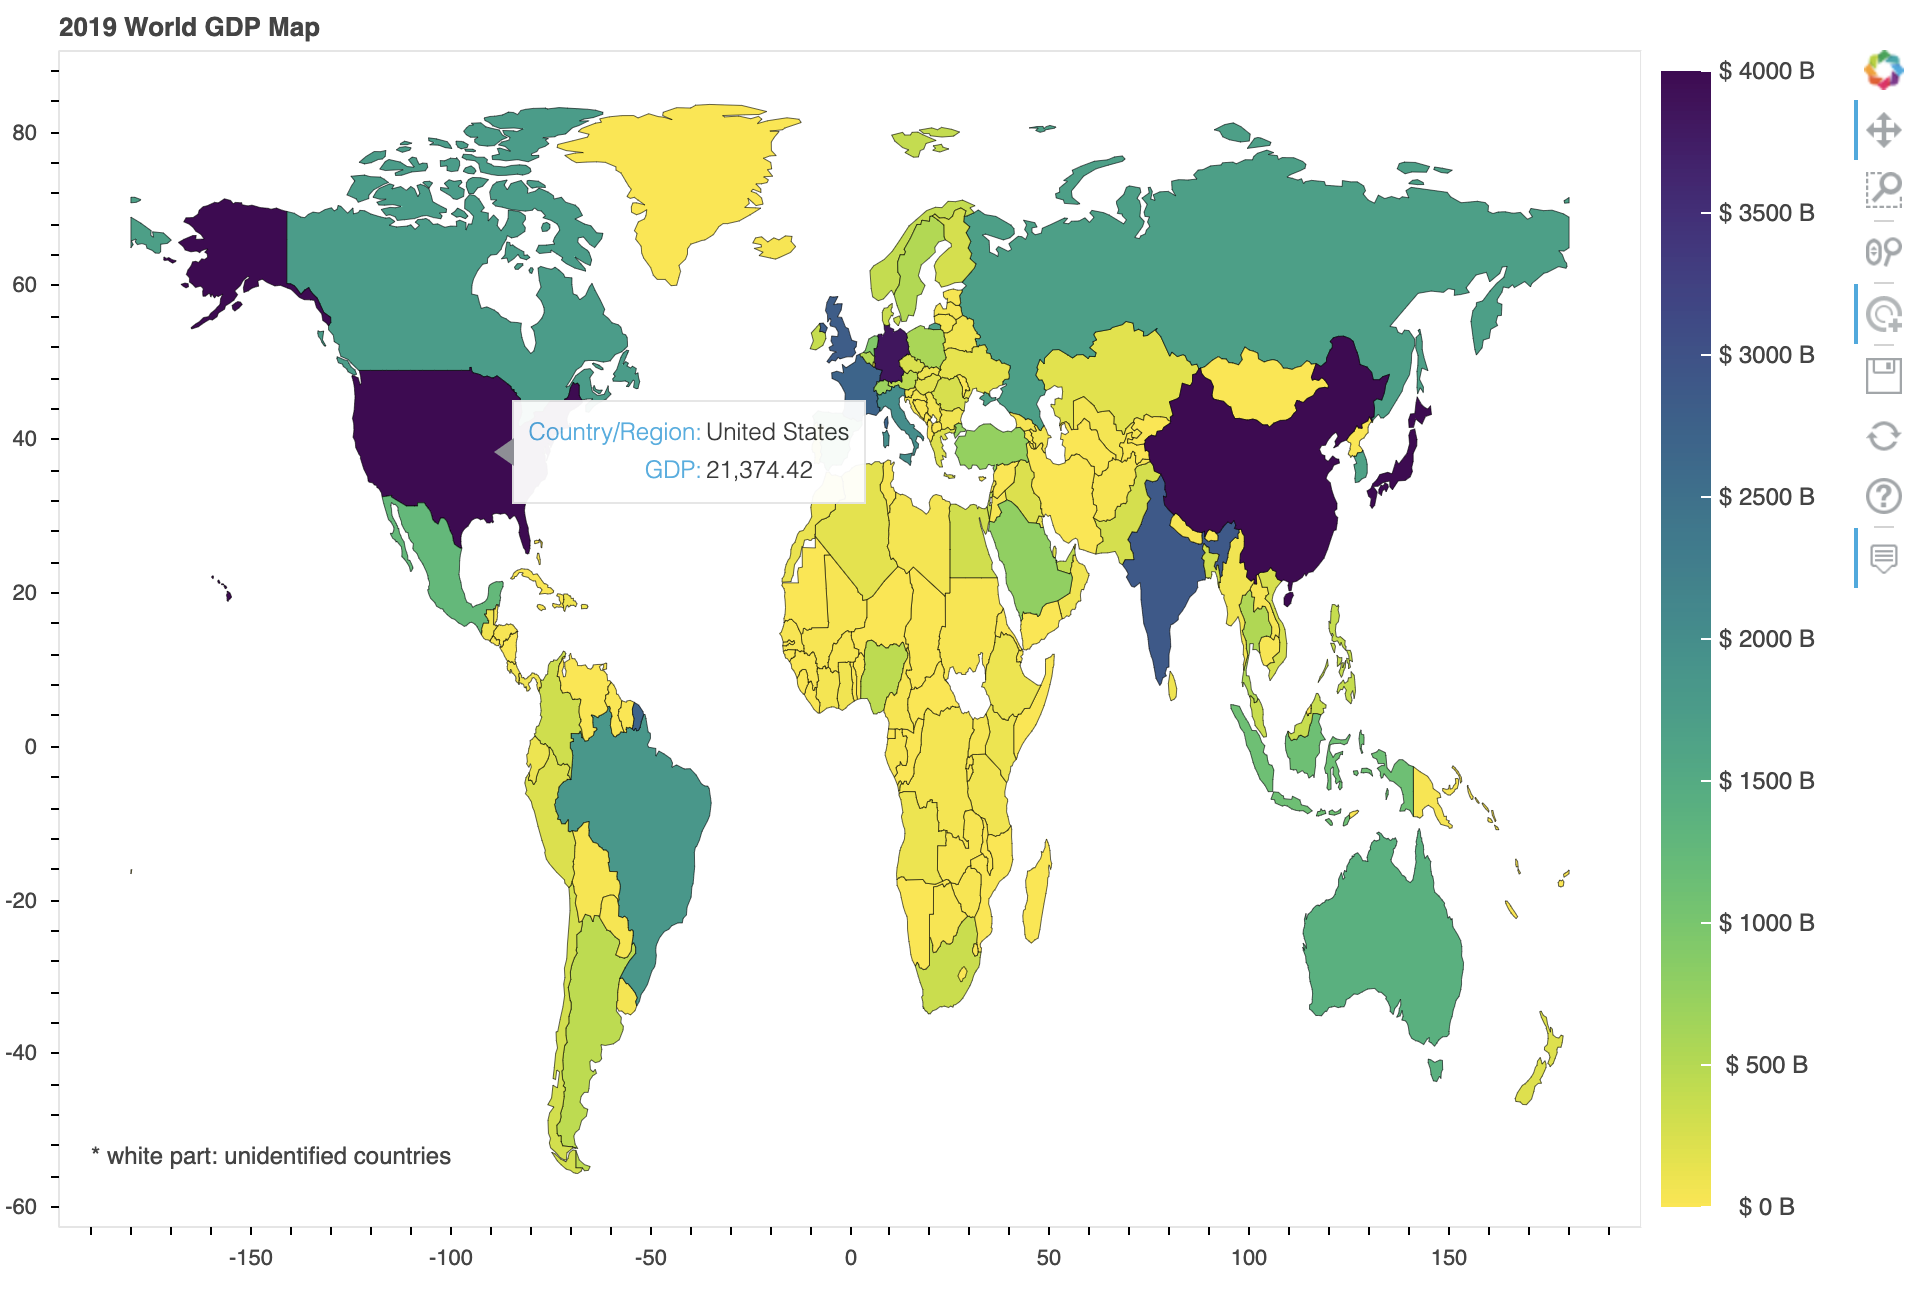
\includegraphics[width=\columnwidth]{hover_gdp.png}
  \caption{Colored GDP world map (unit: \$B). The right column is the continuous linear color bar. Deeper purple indicates higher GDP value and deeper yellow means lower GDP value. When hovering over a particular region, the name of the country and its GDP would be popped up.}
  \label{fig:1}
\end{figure}

Apart from the qualitative display, we also desire the colormap could tell us the quantitative GDP value of a particular country. Display on hover is an intuitive visualization method for this task. Once stopping moving the mouse and hovering over a country, the interface would instantly display the country's name and its GDP value. If we are only interested in a particular region like Europa or countries with small territories like Luxembourg, using wheel zoom tool (the third icon on the tool bar on the right of the color map) could zoom up the desired part easily (shown in \autoref{fig:3}). 


\begin{figure}[tb]
  \centering 
  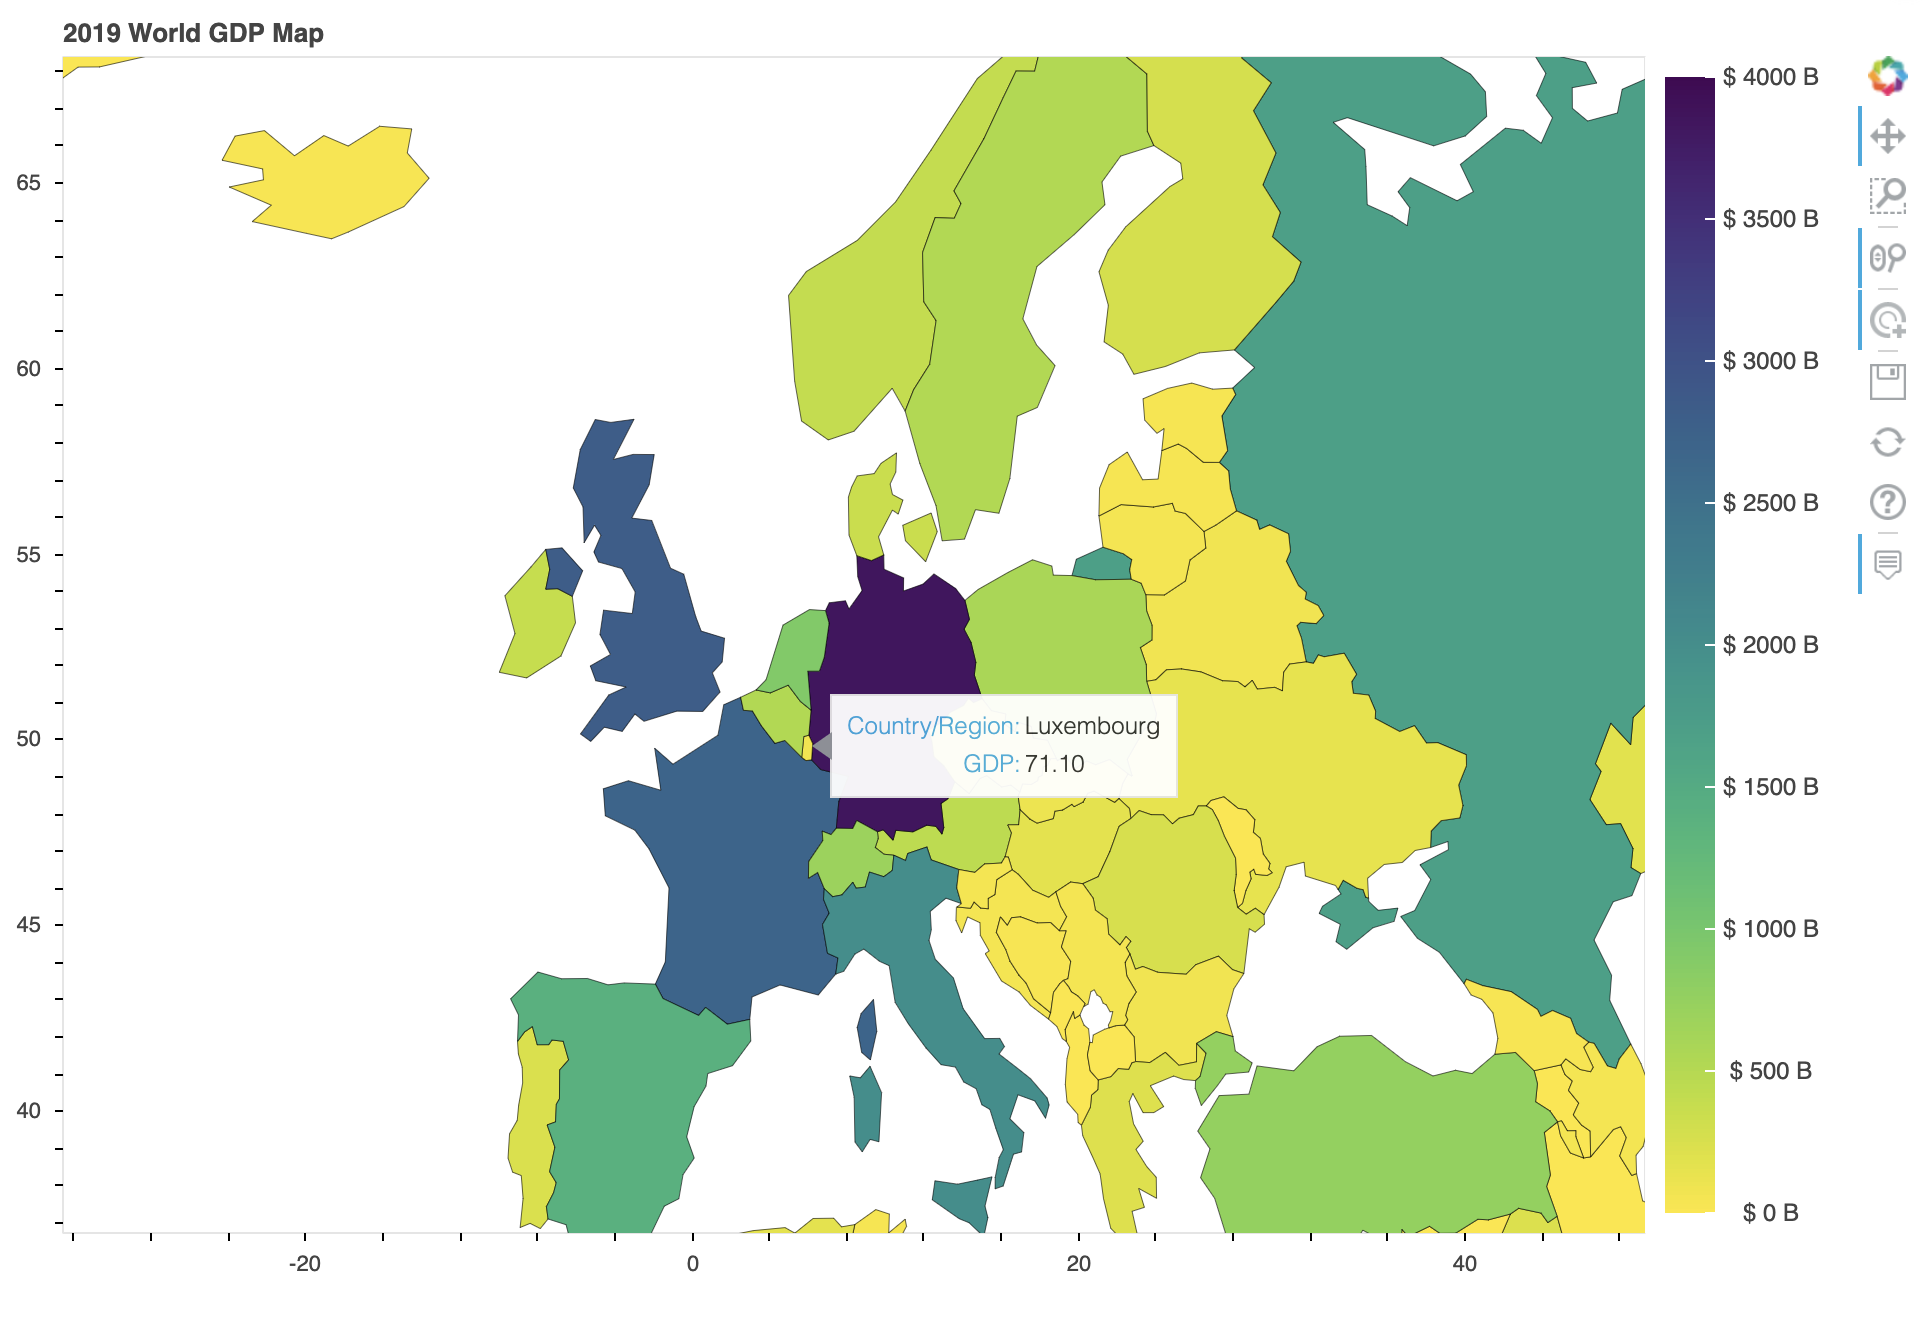
\includegraphics[width=\columnwidth]{gdp_fig5.png}
  \caption{Zoomed GDP color map (Europa region).}
  \label{fig:3}
\end{figure}

\section{Visualization of GDP of Specific Year}
The economic development is a dynamic process. It's necessary for people to learn the economy of a country or the world from the perspective view of history. In order to display the GDP world map in the past year, we design a slider bar on the top of the color map for choosing a value from year 1990 to 2019. As shown in \autoref{fig:4}, after selecting a year we'd like to display, the color map would be regenerated immediately using the GDP data of that selected year. The title of the color map would also be changed corresponding to the selected year. Here is a gif animation figure displaying the GDP development during last 30 years: \textcolor{blue}{\href{https://i.imgur.com/lB4Xoz7.gif}{World GDP map from year 1990 to 2019}}

\begin{figure}[!tb]
  \centering
  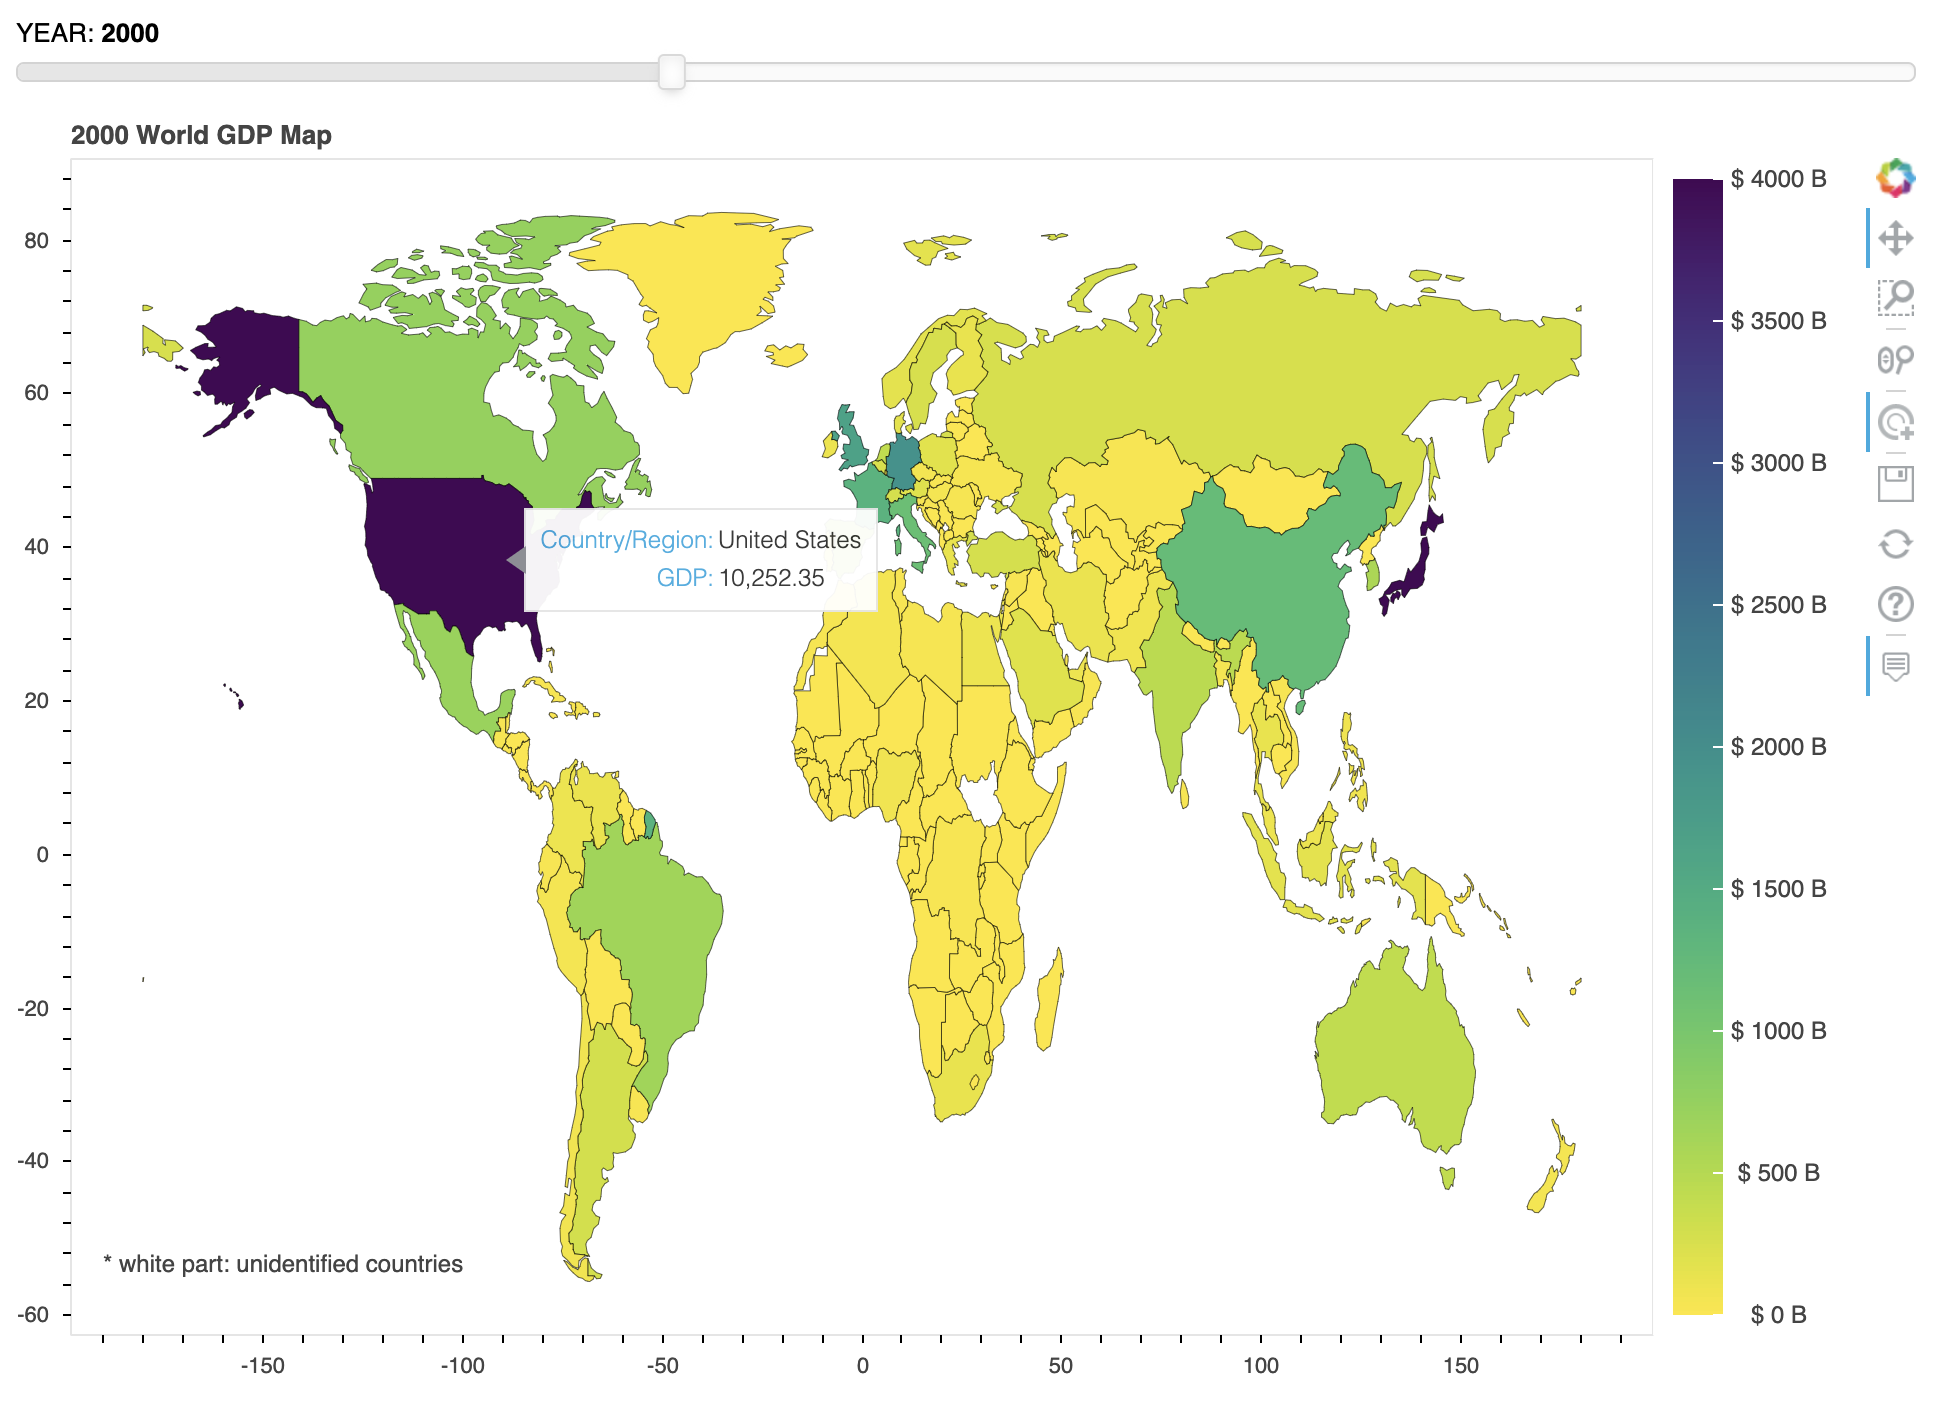
\includegraphics[width=\columnwidth]{hover_slider.png}
  \caption{Visualization of GDP of specific year (year 2000). Top: the slider bar for selecting desired year to display.}
  \label{fig:4}
\end{figure}

\section{Visualization of GDP of Particular Countries}
Since we care more about the economic development trend, it's important to learn the economy change pattern of a particular country during the last 30 years. By comparing the development trend between countries, we could screen both continuously-growing economy and stagnant economy. By learning policies from the former one and alleviating similar issues as the later one, policy-makers could optimize their tools and directions to achieve future progress. In order to display last 30 years' GDP data simultaneously along with the color map, we add an extra widget on the bottom of the color map to visualize data in scatter plot. As shown in \autoref{fig:5}, when we click the target country that we want to view its development trend, only this country would remain highlighting on the color map while the rest countries are blurred in semitransparent. The window on the bottom of the color map would display the GDP values using scatter plot. Besides, the spot color would turn purple and the detailed GDP value of a particular year would be popped up when the mouse is hovering over a specific spot in the scatter plot. With the help of the interactive scatter plot, it's easy to know the development trend of a country. For example, we know that the United States keeps increasing while the Russian Federation experienced economic recession in early 1990s and after year 2014. 

\begin{figure}[tb]
  \centering
  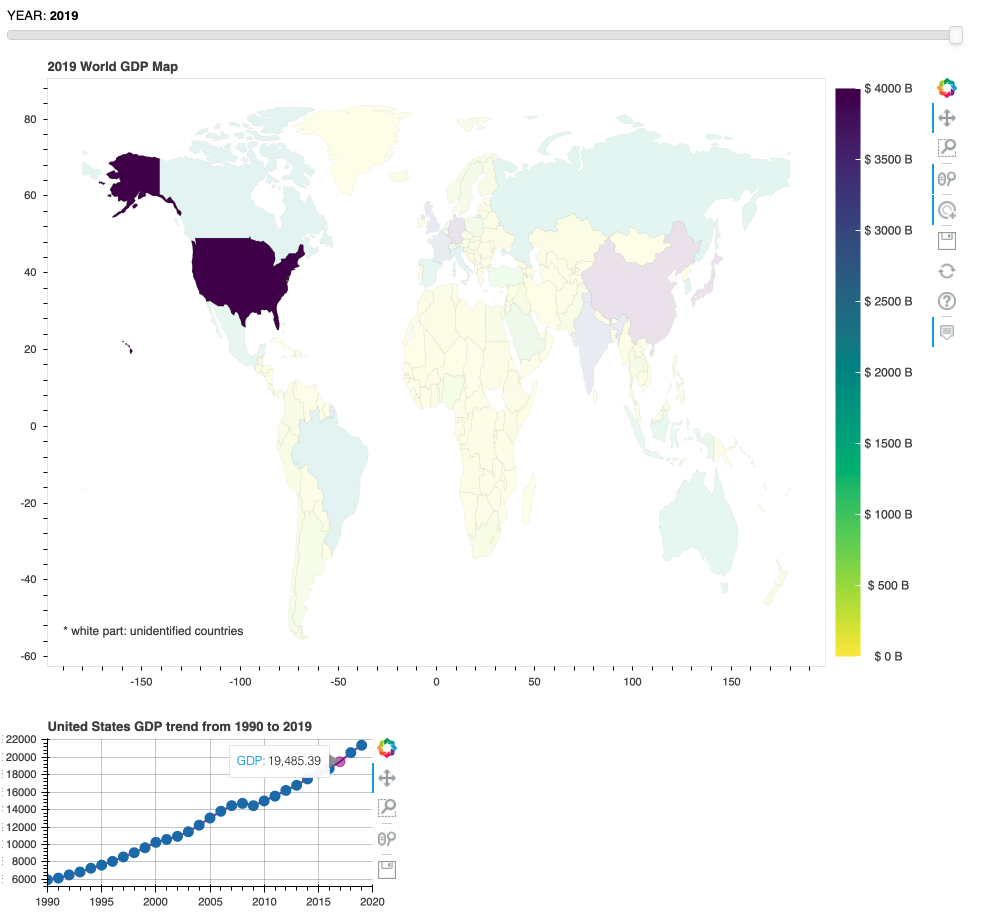
\includegraphics[width=\columnwidth]{gdp_fig6.png}
  \caption{GDP development trend of a particular country (The United States). The bottom scatter plot shows the GDPs over the last 30 year.}
  \label{fig:5}
\end{figure}

\section{Conclusion}
Understanding economic development is an interesting topic. Discerning patterns from the large amounts of historical GDP data is an important but challenging work. In this project, we develop an interactive interface which could help people easily get not only detailed quantitative data but also intuitive qualitative trend information. We hope this tool could help people to conduct visual analytics conveniently or inspire other developer to extend the toolset with more diverse functions. 


\bibliographystyle{abbrv-doi}
\bibliography{project_cs519}
\end{document}
